\documentclass[
]{thesis-ekf}
\usepackage[T1]{fontenc}
\PassOptionsToPackage{defaults=hu-min}{magyar.ldf}
\usepackage[magyar]{babel}
\usepackage{mathtools,amssymb,amsthm,pdfpages,listings}
\footnotestyle{rule=fourth}
\DeclareMathOperator{\arcctg}{arcctg}
\newtheorem{tetel}{Tétel}[chapter]
\theoremstyle{definition}
\newtheorem{definicio}[tetel]{Definíció}
\theoremstyle{remark}
\newtheorem{megjegyzes}[tetel]{Megjegyzés}

\begin{document}
	\institute{Matematikai és Informatikai Intézet}
	\title{A mesterséges intelligencia alkalmazási lehetőségei a haderőben}
	\author{Dobozy Dániel\\programtervező informatikus}
	\supervisor{Dr. Tómács Tibor\\egyetemi docens}
	\city{Eger}
	\date{2023}
	\maketitle
	\tableofcontents
	
	
	\chapter*{Bevezetés}
	\addcontentsline{toc}{chapter}{Bevezetés}
	
	Az elmúlt évtized során az információs technológiákat célzó tudományos fejlődés, illetve az azokból fakadó technológiai modernizáció eredményeképpen felforgató változásnak lehettünk szemtanúi, amely a jövő technológiai lehetőségeit oly mértékben átformálta, hogy az adott kor technológiai szintjén képességek birtokosává válni kívánó szereplőktől folyamatos fejlődést, technológiakövetést, bizonyos technológiai területeken pedig -- amelyek közül kiemelt a mesterséges intelligencia -- folyamatos fejlesztést követel. Alapvetően a műszaki megoldások folyamatos evolúciója tette lehetővé ezt a változást, melynek során az elektronikai alkatrészek technológiájában egyre újabb és újabb digitális jelfeldolgozó processzorok folyamatosan egyre kisebb méretekben és egyre olcsóbban váltak elérhetővé, miközben az új processzorok egymást követő generációi a rohamosan növekvő jelfeldolgozási kapacitásaik, sebességük miatt korábban elérhetetlennek tűnő számítási képességet tettek egyre könnyebben hozzáférhetővé mindenki számára. A rendelkezésünkre álló hatalmas, többnyire feldolgozatlan adatmennyiség az információs technológiához kötődően időszakonként újabb és újabb ,,hot topic''-okat eredményez, melyekre mind a tudományos élet szereplőinek, mind az ipari szférának újabb és újabb megoldásokat kellett keresnie, kidolgoznia.
	
	%12. feladat
	\begin{definicio}\label{def:ai}
		A Mesterséges Intelligencia (MI) az a terület, amely a számítógépek által végzett feladatokra és tevékenységekre utal, amelyeknek általában emberi intelligenciához köthetőek.
	\end{definicio}
	
	Ez a kutatási terület az elmúlt évszázad második felében indult fejlődésnek, és eleinte a ,,nagy mennyiségű adatok'' (\emph{Big-Data}) feldolgozására fókuszált, ráirányítva a figyelmet arra a területre, hogy a gigantikus mennyiségű adatot a korábbi megoldásainkkal nem lehetett hatékonyan kezelni és feldolgozni. Hamarosan erre a problémahalmazra felültetve erősödött fel a ,,gépi tanulás'' (\emph{Machine Learning}) lehetőségeinek kérdése, illetve kapott az utóbbi időben egyre nagyobb figyelmet az MI (\Az \emph{\ref{def:ai}.~definíció}) tudományterülete is, mely a közeljövőben minden, a műszaki tudományterület jelenleg aktív, fontosabb szereplői, így a haderő számára is várhatóan kihívásokat fog jelenteni.
	
	Az MI területének a felkapottsága az utóbbi 3-4 év technológiai fejlődésének eredményeként különösen felerősödött. A jelenlegi fejlesztésben a civil piaci szereplők mellett óriási szerepet kapnak a katonai alkalmazási lehetőségek kutatói is, és ebből adódóan  a kormányzati erőfeszítések egyre szélesebb spektrumban keresik és találják meg a kutatási témák irányait.
	
	%13. feladat
	\Az \emph{\ref{chapter2}.~fejezet} a témára vonatkozó fontos  részleteket tartalmazza.
	\Az \emph{\pageref{chapter2}.~oldalon} kezdődik a fejezet.
	
	\chapter{Az amerikai stratégia előzményei}
	\section{Az amerikai technológiai fölény átalakulása}
	
	%14. feladat
	Ez egy példa szöveg, amely tartalmaz lábjegyzeteket.\footnote{Ez az első lábjegyzet, amely teljes mondatból áll.}
	Itt van egy másik mondat, amely szintén tartalmaz egy lábjegyzetet.\footnote{Ez pedig a második lábjegyzet, ugyancsak egy teljes mondat.}
	
	A hidegháború vége óta az Amerikai Egyesült Államok a nemzet\-közi rendben gyakorlatilag egyedüli szuperhatalomnak tekinthető. Ennek egyik fontos pillére a páratlan katonai technológiai fölény. Az amerikai katonai erőfölényt a múltban alátámasztó technológiák azonban -- mint például a precíziós irányítású fegyverek -- a versenytársak számára is elérhetővé váltak. Kína és Oroszország is olyan képességeket fejlesztett ki, amelyek egyre inkább kihívást jelentenek az amerikai katonai fölénnyel szemben. Kína kutatásai az MI területén elsősorban a gyorsabb és tájékozottabb döntéshozatal elősegítésére, valamint az autonóm katonai járművek kifejlesztésére koncentrálnak, Oroszország MI-fejlesztései pedig elsősorban a robotika területére fókuszálnak.

	Az Amerikai Egyesült Államok Védelmi Minisztériuma először 2016-ban adta ki az MI stratégiáját, melyet első ízben 2018-ban vizsgáltak felül.\footnote{US Department of Defense: Summary of the 2018 Artificial Intelligence Strategy – Harnessing AI to Advance our Security and Prosperity.} A kiadott dokumentumok egyértelműen leírják, hogy ezen a műszaki területen a főbb versenytársaik (Kína és Oroszország) olyan erős kutatási folyamatokat indítottak be, melyek elengedhetetlenné teszik a téma kiemelt kezelését az amerikai stratégiában is.

	\section{Az MI stratégia kiemelése az amerikai védelemben}
	A 2018.~évi védelmi stratégia arra hívja fel a figyelmet, hogy az MI valószínűleg megváltoztatja a háború jellegét.\footnote{US Department of Defense: Summary of the 2018 National Defense Strategy – Sharpening the American Military’s Competitive Edge.} A kormányzati MI-prioritások erősödésével több szinten is szervezeti módosításokat hajtottak végre, így többek között a DARPA\footnote{Defense Advanced Research Projects Agency.} mellé -- amely kifejezetten a védelmi szféra kutatószervezete -- erre a célra egy új kutatóközpont (IARPA\footnote{Intelligence Advanced Research Projects Activity.}) létrehozásáról intézkedtek, melynek felelősségi körébe az MI területéhez kapcsolódó kutatás-fejlesztési témák vezetése tartozik.
	
	A védelmi szektorban a 2016 októberében Ashton Carter védelmi miniszter által létrehozott Védelmi Innovációs Tanács (DIB\footnote{Defense Innovation Board.}) kiemelt ajánlásaként szerepelt egy ,,központosított, koncentrált, jól finanszírozott szervezet létrehozása a Védelmi Minisztériumban, amely a mesterséges intelligencia és a gépi tanulás lehetőségeinek vizsgálatára fókuszál''. Az ajánlás alapján 2018.~június végén megalapították az Összhaderőnemi Mesterségesintelligencia-központot (JAIC\footnote{Joint Artificial Intelligence Center.}).
	
	A JAIC az Amerikai Egyesült Államok Védelmi Minisztériumának MI-központ Kiválósági Központja, amely szakembereivel segítheti a haderő mesterséges intelligencia alkalmazására irányuló törekvéseinek megvalósítását, és célja a haderőn belül a mesterséges intelligenciával kapcsolatos problémák megoldása, valamint a megoldások elterjesztése, elsősorban a missziós feladatok végrehajtása során.
	
	A Pentagon által 2018.~június 27-én kiadott memorandumban\footnote{Memorandum. Subject: Establishment of Joint Artificial Intelligence Center. 27. 06. 2018.} a védelmi miniszter helyettese -- Patrick M. Shanahan -- meghatározza a JAIC konkrét feladatait és a Védelmi Minisztérium információs főnökének alárendeltségébe utalja a szervezetet. Az új szervezet elsődleges feladatként a mesterséges intelligenciával összefüggő katonai kutatások összehangolását, felgyorsítását, illetve kutatási, oktatási és civil programok becsatolását, valamint új partnerek felkutatását kapta.
	
	A memorandum szerint a JAIC átfogó célja, hogy felgyorsítsa a mesterséges intelligenciára épülő képességek kialakítását. Figyelemre méltó, hogy a JAIC középpontjában az etika, a humanitárius megfontolások, valamint a rövid és a hosszú távú MI-biztonság is szerepelnek.
	
	Az elképzelések szerint a JAIC globálisan fontos modellként szolgálhat más hasonló technológiákat alkalmazó szervezetek számára, amennyiben bizonyítja, hogy a biztonságtudatos és etikai megközelítés az MI-hoz nem veszélyezteti a nemzetbiztonságot.
	
	A JAIC tevékenysége nyomán, illetve vele együttműködve az Amerikai Szárazföldi Haderő 2018-ban megalapította a JAIC MI kutatási tevékenységének támogatására a Szárazföldi Mesterségesintelligencia-kutató Központot (Army Artificial Intelligence Task Force in Support of the Department of Defense Joint Artificial Intelligence Center), amelyet egy 2018.~október 2-án kelt memorandumban jelentettek be.
	
	A Központ tevékenységének az alapját a Védelmi Minisztérium MI-stratégiája\footnote{US Department of Defense: Summary of the 2018 Artificial Intelligence Strategy – Harnessing AI to Advance our Security and Prosperity.} és a védelmi miniszter helyettese által kiadott memorandum\footnote{Memorandum. Subject: Establishment of Joint Artificial Intelligence Center. 27. 06. 2018.} jelentették. Az új szervezet célja elősegíteni a jelenlegi technológiák alkalmazásának javítását és csökkenteni az MI-képességek hiányát, ezzel is segítve a béke megőrzését vagy a győzelem kivívásának lehetőségét.
	
	A Kongresszusi Kutatószolgálat (CRS\footnote{Congressional Research Service.}) 2019 elején frissítette a mesterséges intelligenciával és a nemzetbiztonsággal foglalkozó összefoglalóját, amelyből további részletek derülnek ki az amerikai kutatási programokról.
	
	A CRS hiteles, bizalmas és objektív politikai és jogi elemzéseket biztosít a bizottságok, a parlament és a Szenátus tagjai számára, függetlenül a pártoktól. A Kongresszusi Könyvtár jogalkotói ügynökségeként a CRS több mint egy évszázadig értékelt és tiszteletben tartott erőforrás volt a politikai döntéshozói körökben, és azt támasztja alá, hogy a mesterséges intelligenciával kapcsolatos amerikai kutatások és fejlesztések a kínai és az orosz nyilatkozatokra és tervekre reflektálnak.
	
	\section{Az MI stratégia és az amerikai védelem új kihívásai}
	Konkrétumokról nyílt forrásból elég keveset lehet hallani, de viszonylag széles körű nyilvánosságot kapott az egyik úttörő 2017-es projekt,\footnote{CNN: ,,Project Maven''.}
	amelynek során az MI segítette az Iszlám Állam elleni harcot Irakban és Szíriában. A Maven-projekt fő területeit az információgyűjtés és -elemzés, a logisztika, a számítógépes műveletek, az információs rendszerek üzemeltetése, irányítása, ellenőrzése, valamint a különböző autonóm és félautonóm járművek alkalmazásai jelentették.
	
	A védelmi szféra már az elmúlt években is számos lehetséges problémát vetett fel. Ezek költségeinek fedezésére a Pentagon már 2017-ben jelentős összegeket tervezett, és a következő lényeges kérdésekre kereste a választ:
	\begin{itemize}
	\item Mi a megfelelő arány a katonai MI-fejlesztéseknél a kereskedelmi és kormányzati finanszírozás tekintetében?
	\item Hogyan befolyásolja döntéseivel a Kongresszus a katonai MI-fejlesztéseket?
	\item Milyen változások szükségesek az ellenőrzés területén (Kongresszus és Védelmi Minisztérium)?
	\item Milyen etikai megfontolásokat kell figyelembe venni (és egyensúlyba hozni) az MI-fejlesztések és az autonóm rendszerek esetében?
	\item Milyen jogalkotási változások szükségesek a katonai MI-alkalmazások tekintetében?
	\item Milyen intézkedéseket hozhat a Kongresszus, hogy segítse az MI-verseny globális kezelését?
	\end{itemize}




\chapter{A mesterséges intelligencia stratégiai programja}\label{chapter2}
A 2018-ban kiadott stratégia első és legfontosabb üzenete az, hogy az Amerikai Egyesült Államok Védelmi Minisztériuma azonnali lépéseket akar tenni a mesterséges intelligencia lehetséges előnyeinek kihasználására. 

%10. feladat
\begin{figure} [h]
	\centering
	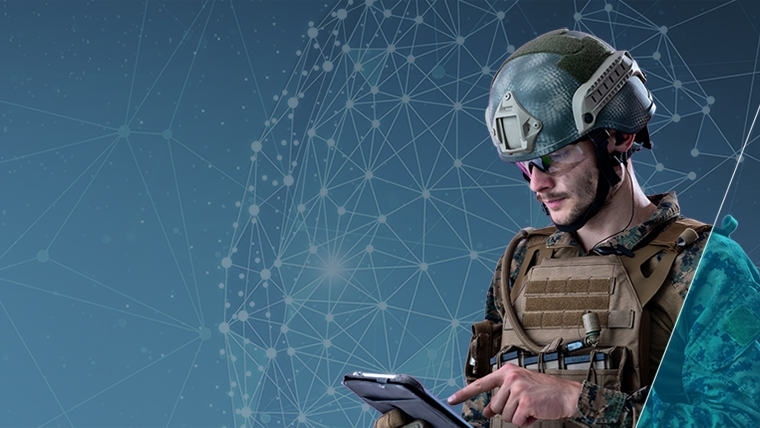
\includegraphics[width=5cm]{AI.png}
	\caption[]{A MI alkalmazási lehetőségei a haderőben}
	\label{fig:ai-kep}
\end{figure}

Ennek érdekében szerveztek egy sor kezdeményezést, amelyek azt célozták, hogy az MI gyorsan, iteratívan és felelősségteljesen beépüljön a katonai döntéshozatalba a missziós területen folytatott műveletek hatékonyabbá tétele érdekében. A minisztérium azt is meghatározta, hogy ezek a kezdeményezések milyen konkrét feladatokat foglalnak magukban, és azok milyen kulcsfontosságú platformokon keresztül valósíthatók meg. Ezek között szerepel a közös alapokon nyugvó adatok megosztásának lehetősége, az újrafelhasználható eszközök létrehozása, a szabványok pontosítása, a felhő- és a széles sávú szolgáltatások elérésének szabályozása. Ezzel párhuzamosan lépéseket határoztak meg az MI-alkalmazások folyamatainak előkészítésére digitalizálással és intelligens automatizálással.


\section{Stratégiai irányok}
A stratégia módosítása alapvetően nyolc irányt rögzített:

%11. feladat
\begin{enumerate}
	\item \emph{Hosszú távú beruházások szükségesek} az MI-tárgyú K+F-területen, ezek elsődlegesen kerülnek végrehajtásra, és a prioritásokat a költségvetés tervezésénél is figyelembe kell venni.
	\item Kiemelt terület a hatékony \emph{megoldások fejlesztése az ember és az MI együttműködésének optimalizálására}.
	\begin{enumerate}
		\item A fő fókusz a kapcsolathoz szükséges kommunikáció és a valós helyzetkép átadhatóságának kérdése.
		\begin{enumerate}
			\item[---] Erős fejlesztésre van szükség például a vizualizációs technikák, a hatékony nyelvfeldolgozás és az emberi képességek kiegészítését biztosító technológiák területén.
		\end{enumerate}
	\end{enumerate}
	\item Az \emph{MI-rendszerek etikai, jogi és társadalmi vonzatainak fejlesztése} olyan megoldások keresése, amelyek ezt a kérdéskört támogatni képesek.
	\begin{enumerate}
		\item Ez egy rendkívül összetett, több tudományterület ötvözését igénylő feladat.
	\end{enumerate}
	\item Az \emph{MI-rendszerek biztonságának, védelmének erősítése} olyan MI-alapú rendszerek fejlesztését kell megcélozni, melyek biztonságosak, ellenállók, megbízhatóak és hitelesek.
	\begin{enumerate}
		\item Ezeket a követelményeket a fejlesztéseknél érvényesíteni kell ahhoz, hogy a technológia ténylegesen hasznosítható lehessen.
		\begin{enumerate}
			\item[---] Ehhez olyan kutatási témákat indított a DARPA és az IARPA, melyek az MI-rendszerek, illetve a velük szembeni követelmények pontosításához a megbízhatóságot, a támadások elleni sebezhetetlenségek erősítését és ezek hitelesítését irányozzák elő.
		\end{enumerate}
	\end{enumerate}
	\item Megosztott, \emph{nyilvános adatkészlet és környezet fejlesztése} oktatásra és tesztelésre, vagyis a fejlesztések és az oktatás nem fog tudni működni a megfelelő környezet elérhetősége nélkül.
	\begin{enumerate}
		\item Erre szövetségi és a részt vevő ipari, illetve szolgáltatói szereplők biztosítanak hozzáférést a rendelkezésre álló adathalmazokból nagy mennyiségű adatokhoz (közlekedési szenzoroktól származó adatok, egészségügyhöz kapcsolódó adatok stb.).
	\end{enumerate}
	\item Az \emph{MI-technológiák mérése és értékelése} azaz szabványokon és egységes mérőszámokon alapuló mérések végrehajtása során ki kell alakítani a megoldások széles spektrumát az összehasonlításhoz, a független értékeléshez.
	\begin{enumerate}
		\item Ehhez egyrészt fejleszteni kell a standardok kialakíthatóságát, másrészt erőfeszítéseket kell tenni egy mérőszámokon alapuló összehasonlíthatóság, értékelhetőség kialakításához.
		\begin{enumerate}
			\item[---] Fejleszteni kell az MI-környezeteket a kutatók munkájának segítésére.
		\end{enumerate}
	\end{enumerate}
	\item Az \emph{MI területén aktív fejlesztők szükségleteinek} jobb megértése és fejlesztése, vagyis lehetőség szerint fejleszteni szükséges a nemzeti K+F-képességet, és kiemelt hangsúlyt kell fektetni a fejlesztő- és kutatóállomány toborzására és megtartására.
	\item Az MI fejlesztése érdekében \emph{fejleszteni kell a kapcsolatrendszert a nyilvános szereplőkkel}, azaz minél szélesebb körű érdekeltséget kell elérni, mert rendkívül széles a technológiai terület, továbbá a kutatási befektetések döntő hányada nem a kormányzati szektorból jön, így az eredmények érdekében az erőfeszítéseket össze kell hangolni.
\end{enumerate}

%16.feladat
\begin{equation} \label{keplet}
	h: R\,\backslash\left\{\frac{\pi}{3}k:k\in\mathbb{Z}\right\} \to \mathbb{R},\quad h(x) :=
	\begin{cases}
		\frac{\arcctg(x+2\pi)}{\sin(3x)},& \text{ha }x \leq - \frac{2}{3},\\
		\lg^{3}(3x+2),& \text{különben. }
	\end{cases}
\end{equation}

A képletre itt \emph{\ref{keplet}} lehet hivatkozni.

\section{Konkrét Területek az MI Alkalmazásában}
A kiadott stratégia részletesen foglalkozik a megvalósítás kérdéseivel is. Azon belül kiemelt kérdésként tárgyalja, hogy milyen kulcsfontosságú küldetésekkel kell foglalkozni az MI-képes funkciók megvalósításával. Ezek a területek nemcsak a missziós tevékenységekre terjednek ki, de felölelik a békevezetés területeit is. A stratégia szerint az MI-alkalmazások lehetséges területei:

\begin{itemize}
	\item A \emph{helyzettudatosság és a döntéshozatal javítása}. Ebbe a körbe tartoznak azok az MI-alkalmazások, amelyek képesek a vezetőket ellátni helyzetinformációkkal (pl.~képelemzés), ezáltal segítve az optimális cselekvési utak kiválasztását, tehát a döntéshozatalt.
	\item A \emph{műveletbe bevont eszközök, berendezések biztonságának növelése}. Lényegében meg kell teremteni a lehetőséget az MI segítségével, hogy a bonyolult helyzetekben is fokozzák a repülőgépek, a hajók és más járművek biztonságát azáltal, hogy az MI figyelmeztetést küld az üzemeltetőknek.
	\item A \emph{prediktív karbantartás és ellátás megvalósítása}. Az adatokra és a berendezések állapotára alapozva az MI-t használjuk a kritikus alkatrészek meghibásodásának előrejelzésére, a diagnosztika automatizálására és a karbantartás megtervezésére. Hasonló technológiákat fognak használni a pótalkatrészek készítésének irányítására és a készletszintek optimalizálására. Ezek az előrelépések biztosítják a megfelelő készletszinteket, segítenek a hibaelhárításban, valamint lehetővé teszik alkalmazkodó erők gyorsabb és olcsóbb telepítését. A végrehajtás úgy történhet, hogy a mesterséges intelligencián alapuló megoldások az egyedi berendezések vezérlőjén keresztül gyűjtik össze, elemzik és használják fel az adatokat, hogy meghosszabbítsák a berendezés élettartamát és a leállások megelőzése érdekében észleljék a hibákat. A nyers adatok begyűjtésének folyamatát már automatizálták, és ezt már teljes egészében a gépeken belül az ,,\emph{Edge}'' mellett működő új, mesterséges intelligencián alapuló vezérlő végzi az adatok megbízhatóságának és egységességének érdekében. Ráadásul a vezérlő az összefüggések elemzése alapján automatikus adatmodellezést végez és ellenőrzi a berendezés állapotát.
	\item A \emph{végrehajtás egyszerűsítése}. Az MI-t azzal a céllal fogják használni, hogy csökkentse a manuális, ismétlődő és gyakori feladatokra fordított időt. Az automatizált feladatok felügyeletének lehetővé tétele révén az MI képes csökkenteni a hibák számát és így a költségeket, növelni a teljesítményt és a mozgékonyságot, valamint előmozdítani a  Védelmi Minisztérium erőforrásainak elosztását magasabb értékű tevékenységekre és a feltörekvő missziós prioritásokra.
	
	%18. feladat
	\cite{AllenChan,Goodfellow}
\end{itemize}

%17. feladat
\lstinputlisting[
language=C++,
caption={Példa kód},
label=exampleCode,
numbers=left,
numberstyle=\tiny,
keywordstyle=\color{blue}\bfseries,
commentstyle=\color{green},
breaklines=true
]{example.cpp}

A felsorolt konkrét tevékenységeket mintegy akciótervként értelmezve körvonalazódik, hogy milyen alapelveket kívánnak követni az amerikai védelmi szférában az MI-fejlesztések során:

\begin{itemize}
	\item \emph{Átfogó megközelítés}. A társadalom egészét érintő jelentős globális kihívások (humanitárius segítségnyújtás, erdőtüzek, hurrikánok, földrengések, katasztrófák) MI segítségével történő kezelése nyitott MI-küldetések kialakításával. Ezek a feladatok kihívást jelentenek egy széles körű közösség számára, és így összefogva az egyetemeket és az ipar szereplőit elősegítheti a fő védelmi feladatok megvalósítását is.
	\item A \emph{partnerség erősítése a tudományos élet szereplőivel és új MI innovációs körzetek elterjesztése}. A stratégia szerint az egyetemek számára hosszabb távú stabil finanszírozást biztosítanak, hogy a legjobb tudósokat vonzzák a kritikus védelmi területekkel kapcsolatos hosszú távú kutatásba, valamint biztosítsák az MI-fejlesztés területén tehetséges szakemberek következő generációjának oktatását. Ez magában foglalja a meglévő csatornákon – például a DARPA, az IARPA és a haderőnemi kutatólaboratóriumok segítségével történő beruházások növelését, valamint a minisztérium szempontjából releváns hosszú távú felfedezések támogatását.
	\item A \emph{partnerség megerősítése az Amerikai Egyesült Államok iparával}. A stratégia kimondja, hogy az MI-technológia ökoszisztémájának bevonása és megerősítése megköveteli, hogy számos -- tradicionálistól eltérő -- partnerségi modellel kísérletezzenek. Ezek közé tartoznak merész új MI-kezdeményezések nagy ipari partnerekkel, induló kis- és közepes vállalkozásokkal, valamint kockázatitőke-befektetőkkel. Emellett lépéseket tesznek annak érdekében, hogy az MI-közösség tagjai könnyebben részt vehessenek a folyamatokban, például fel kell gyorsítani a fontosabb partnerségi folyamatokat és csökkenteni szükséges az adminisztratív akadályokat. Létrehoznak egy központosított MI-portált a potenciális partnerek számára, amely részletezi a kulcsfontosságú folyamatokat, az érdeklődésre számot tartó témákat és a kapcsolatokat a szerződések és a beszerzés egyszerűsítése érdekében.
	\item \emph{Fejlődő nemzetközi szövetségek és partnerségek}. Kölcsönösen előnyös szövetségek és partnerségek kiterjesztett hálózata az együttműködés révén tartós eszköz a globális MI-kihívások leküzdésére, az agresszió megakadályozására és a stabilitás támogatására. A külföldi szövetségesek és partnerek olyan perspektívákat és tehetségeket kínálnak, amelyek során a résztvevők bevonása, a kombinált portfóliótervezés és az együttműködésen alapuló MI-fejlesztések kiépítéséből származó átjárhatóság bizalmat hozhat létre
	\item \emph{Kapcsolatok ápolása a nyílt forráskódú közösséggel}. A nyílt forráskódú közösség  a tehetséges egyének és átalakító ötletek globális inkubátora. Adatainkat, kihívásainkat, kutatásainkat és technológiáinkat hozzáadva ehhez a közösséghez – a nyílt forráskódú ökoszisztémával együttműködve – ez a leghatékonyabb eszköze a tehetségek bevonzásának, illetve a fejlesztések során törekedni lehet az új védelmi technológiákat átalakító új MI-technológiák azonosítására, valamint az elérhető technológiai bázis bővítésére is. Ez a terület természetesen számtalan biztonsági kérdést generál, amelyek vizsgálatára a stratégia később egy külön részben tér ki.
\end{itemize}

\chapter*{Összegzés}
\addcontentsline{toc}{chapter}{Összegzés}
Az alkalmazási lehetőségek kutatása a mesterséges intelligencia terén rendkívül sokrétű és kiemelkedően fontos a haderő szempontjából. Az ilyen kutatások és fejlesztések átfogó hatást gyakorolnak a katonai tevékenységekre és az ország biztonságára. A mesterséges intelligencia terén elért előrelépések segíthetnek az autonóm rendszerek fejlesztésében, a döntéstámogatás hatékonyságának növelésében, valamint a gépi tanulás alkalmazásában az adatok elemzésére és az információk gyors feldolgozására.

Ezen technológiák alkalmazása lehetővé teszi az új stratégiák kidolgozását, az ellenséges tevékenységek korai észlelését és az azonnali reagálást a változó körülményekre. Az önállóan működő, mesterséges intelligenciával felvértezett eszközök képesek lehetnek az emberi beavatkozás nélküli, precíz működésre, így minimalizálva a kockázatokat és az emberi életek veszélyeztetését a hadműveletek során.

Ezen túlmenően, az ilyen technológiák fejlesztése hozzájárulhat az adatbiztonság növeléséhez és az információs rendszerek védelméhez, ami kritikus fontosságú a modern háborús környezetben. A mesterséges intelligencia alkalmazása a haderőben így nemcsak a katonai tevékenységek hatékonyságát növeli, hanem hozzájárul a nemzet biztonságának és védelmének megerősítéséhez is.

\begin{thebibliography}{7}
	\addcontentsline{toc}{chapter}{\bibname}
	
	\bibitem{AllenChan}
	\textsc{Allen, Greg – Chan, Taniel}: \emph{Artificial Intelligence and National Security}, July 2017. Cambridge, Harvard Kennedy School, Belfer Center. Available at: \url{https://www.belfercenter.org/sites/default/files/files/publication/AI%20NatSec%20-%20final.pdf}
	
	\bibitem{Congressional}
	\textsc{Congressional Research Service}: \emph{Artificial Intelligence and National Security (2019)}, January 30, 2019. Available at: \url{https://crsreports.congress.gov/product/pdf/R/R45178}
	
	\bibitem{DefenseInnovation}
	\textsc{Defense Innovation Board}: \emph{https://innovation.defense.gov}
	
	\bibitem{Goodfellow}
	\textsc{Goodfellow, Ian J. – Pouget-Abadie, Jean – Mirza, Mehdi – Xu, Bing – Warde-Farley, David – Ozair, Sherjil – Courville, Aaron – Bengio, Yoshua}: \emph{Generative Adversarial Nets}, June 10, 2014. Available at: \url{https://arxiv.org/pdf/1406.2661.pdf}
	
	\bibitem{Leung}
	\textsc{Leung, Jade – Fischer, Sophie-Charlotte}: \emph{JAIC: Pentagon debuts artificial intelligence hub}, August 8, 2018. Available at: \url{https://thebulletin.org/2018/08/jaic-pentagon-debuts-artificial-intelligence-hub/}
	
	\bibitem{DoDStrategy}
	\textsc{US Department of Defense}: \emph{Summary of the 2018 Artificial Intelligence Strategy – Harnessing AI to Advance our Security and Prosperity}. Available at: \url{https://media.defense.gov/2019/Feb/12/2002088963/1/-1/1/SUMMARY-OF-DOD-AI-STRATEGY.PDF}
	
	\bibitem{NationalDefense}
	\textsc{US Department of Defense}: \emph{Summary of the 2018 National Defense Strategy – Sharpening the American Military’s Competitive Edge}. Available at: \url{https://dod.defense.gov/Portals/1/Documents/pubs/2018National-Defense-Strategy-Summary.pdf?mod=article_inline}
	
\end{thebibliography}

% Aláírt, szkennelt nyilatkozat beillesztése a szakdolgozat végére
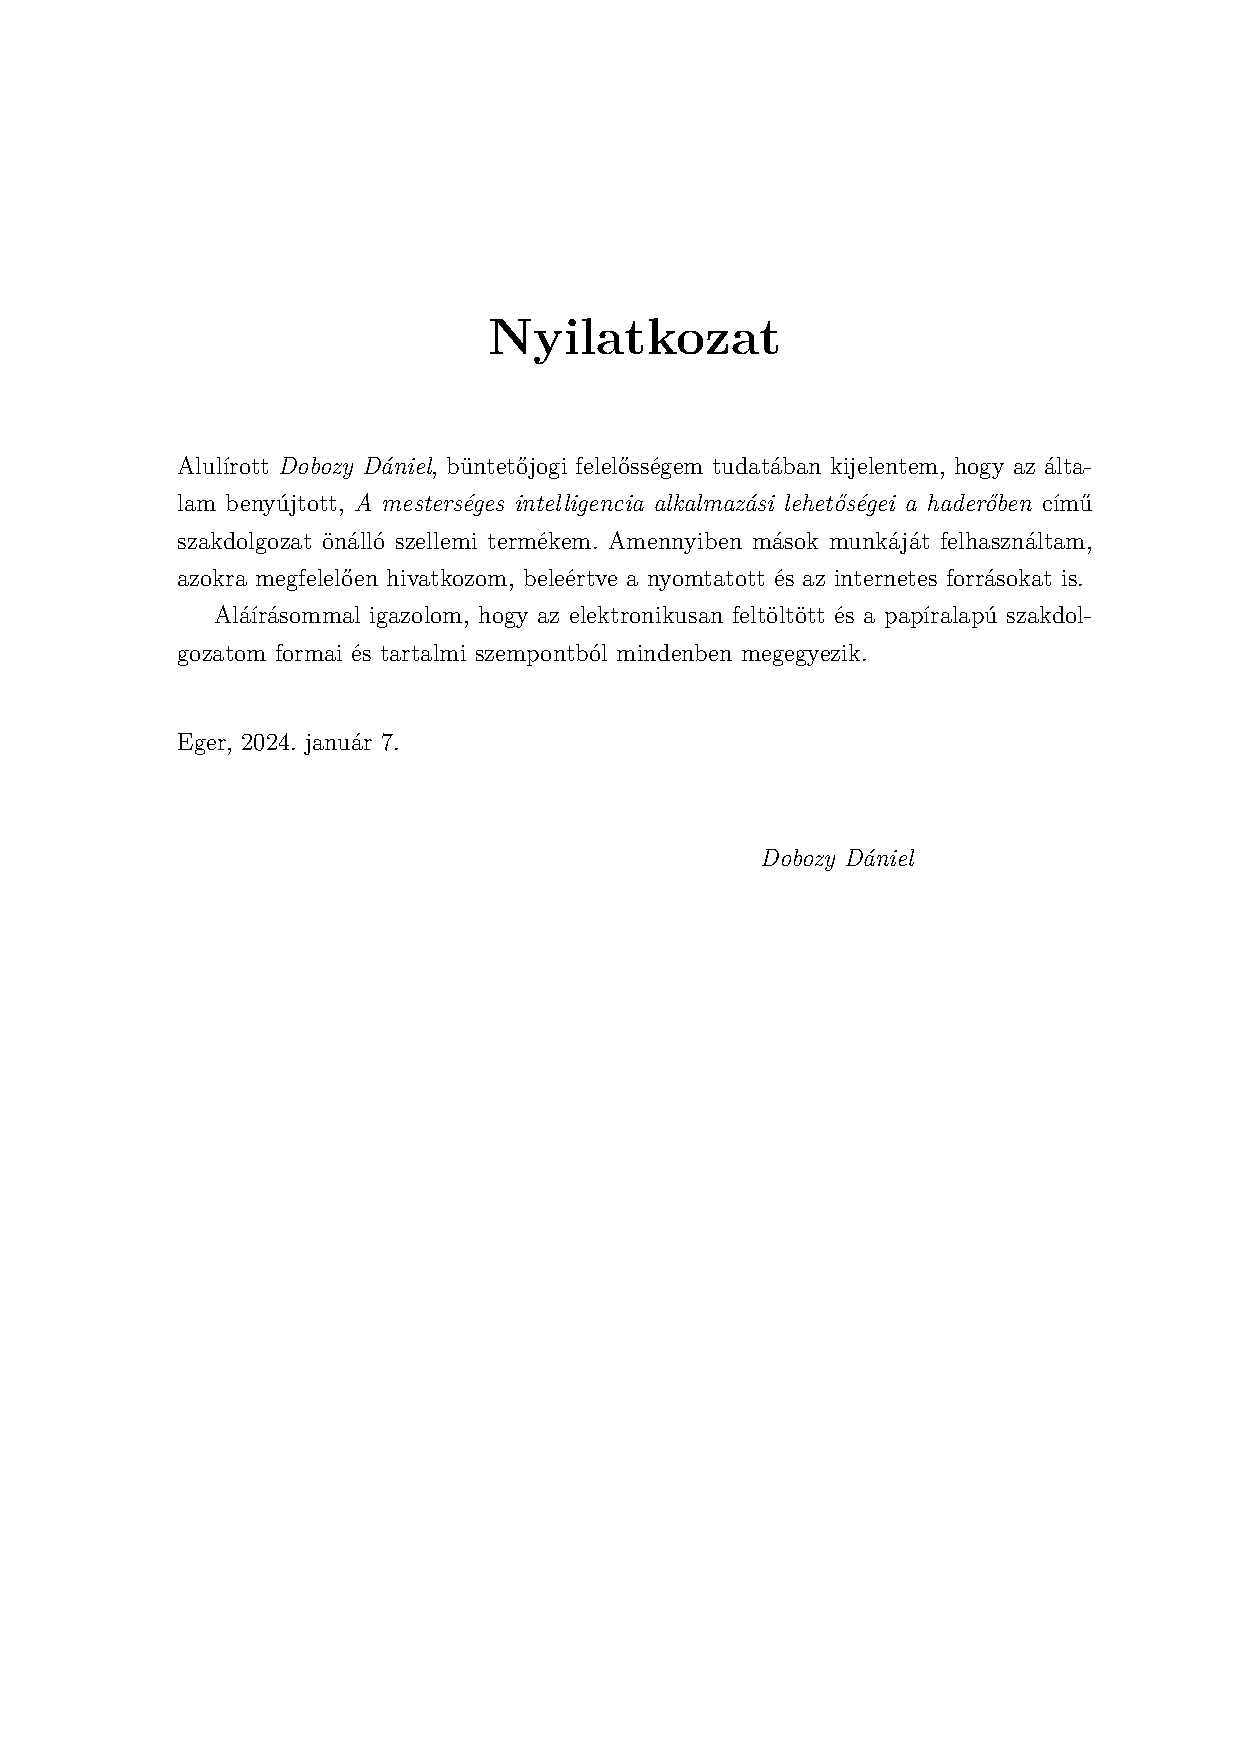
\includepdf{nyilatkozat.pdf}
\end{document}